\begin{figure}
    \centering
    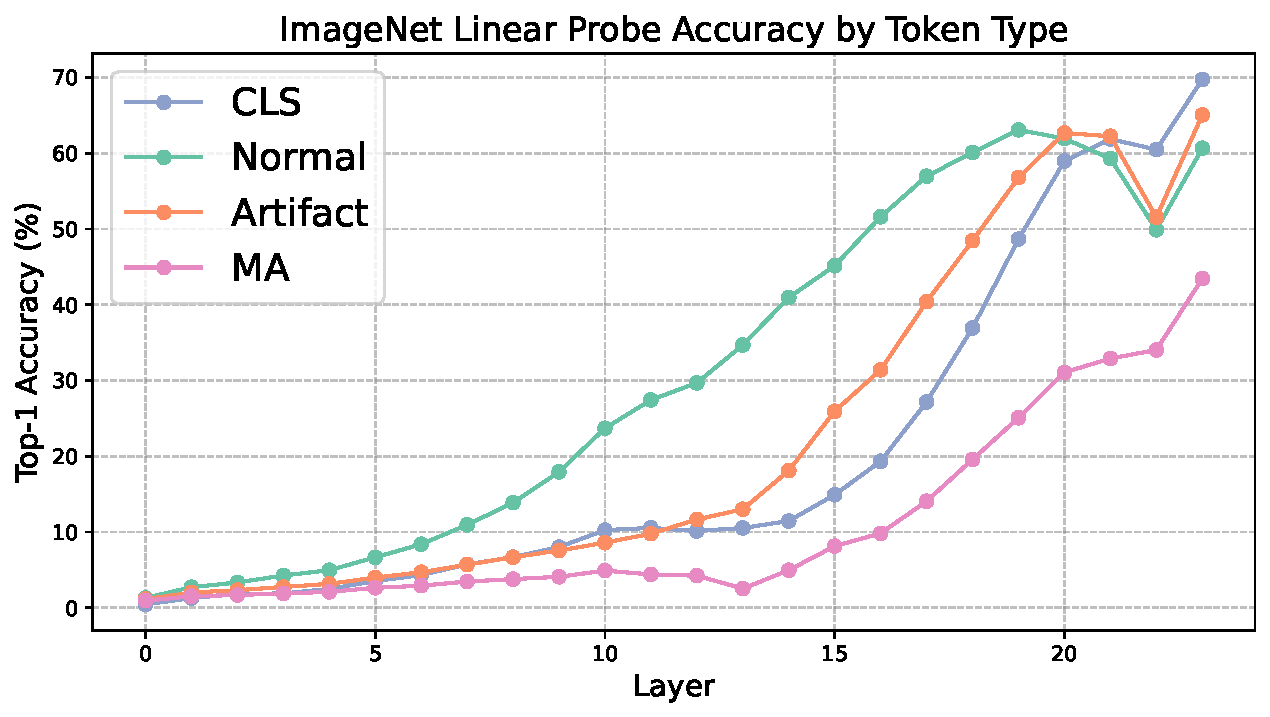
\includegraphics[width=1\linewidth]{figs/imagenet_linear_probe.pdf}
    \vspace{-2em}
    \caption{Fitting a linear probe to the average token grouped by type at each layer shows that CLS tokens contain less global semantic information than Normal tokens until the last layers in CLIP.}
    \label{fig:imagenet_lin_probe}
\end{figure}


\section{Additional Performance Gains}
\label{sec:performance_efficiency}

% We implemented Fast Nystr\"om Attention as a PyTorch module that serves as a drop-in replacement for standard attention. We evaluated our approach on CLIP ViT L-14 \cite{ilharco2021openclip} \cite{radford2021clip} and DINOv2 \cite{oquab2023dinov2} ViT L-14 models without any additional training or fine-tuning. Retrieval performance was assessed on COCO Captions \cite{chen2015coco} and Flickr30k \cite{young2014flickr} datasets using Recall@K metrics for bidirectional text-image retrieval. For vision-specific applications, we conducted zero-shot classification on ImageNet \cite{deng2009imagenet} and linear probing for semantic segmentation on VOC2012 \cite{pascal-voc-2012} and ADE20k \cite{zhou2017ade} datasets. All experiments were performed using a single NVIDIA RTX 4090 GPU.


% \subsection{Efficiency Gains}
% Our experiments show that Nystr\"om attention compression with FPS sampling delivers robust results, whereas approaches like random sampling or $k$-means clustering yield worse results or require retraining, as shown in \cite{xiong2021nystromformer}. In our Fast Nystr\"om Attention method, we guarantee the inclusion of the CLS token in the subsample while using FPS to select the remaining tokens. This approach works effectively because massive and artifacts tokens are statistical outliers on the feature manifold, ensuring that FPS naturally samples these tokens without over-saturating the subsample. In comparison to other sampling methods, we find that this performs near-identically to guaranteeing the sampling of massive tokens, significantly better than guaranteeing the sampling of artifact tokens, and notably better than excluding either. We opt to ignore rather than guarantee massive tokens as it bypasses the need to explicitly extract them and instead relegate that task to the proficiency of FPS. The details of these results are illustrated in Appendix \ref{sec:appendix_performance}.

% There is an intuitive tradeoff between efficiency with smaller sample sizes vs. model performance, but diminishing returns are quickly reached with larger samples. Empirically, we find a sample size of 32 to 64 sufficient to approximate attention with competitive results to standard attention with no additional training required (see Table~\ref{tab:nfa_speed_and_mem}). Results of applying Fast Nystr\"om Attention to vision backbones of CLIP and DINOv2 are shown in Tables \ref{tab:combined_retrieval}, and \ref{tab:vision_only_results}. 

% The main bottleneck of Fast Nystr\"om Attention lies in the FPS sampling step, which reduces the time complexity of the attention mechanism from $O(n^2)$ to $O(ns)$ where $n$ is the input sequence length and $s$ is the sample size. We further optimize performance by sampling once after massive token formation and reusing the same sample mask in the subsequent layers, further reducing the time complexity to $O(n)$. As demonstrated in Tables \ref{tab:combined_retrieval} and \ref{tab:vision_only_results}, this single-sampling approach trades efficiency gains with only a minimal impact on performance metrics. In contrast with standard attention, the memory complexity of FPS sampling remains linear at $O(n)$ regardless of sample size. We compare the runtime speed and memory consumption of Fast Nystr\"om Attention with standard attention in Table \ref{tab:nfa_speed_and_mem}. 

% \begin{table}[H]
% \centering
% \footnotesize
% % Subtable (a): Image Retrieval
% \begin{subtable}[t]{\columnwidth}
% \centering
% \resizebox{\columnwidth}{!}{%
% \begin{tabular}{lcccccc}
% \toprule
%  & \multicolumn{3}{c}{COCO} & \multicolumn{3}{c}{Flickr30k} \\
% Model & R@1 & R@5 & R@10 & R@1 & R@5 & R@10 \\
% \midrule
% CLIP & 35.33 & 59.97 & 70.15 & 65.20 & 87.24 & 92.00  \\
% CLIP+FNA+no resample & 35.42 & 60.18 & 70.27 & 65.17 & 87.22 & 91.95 \\
% CLIP+FNA+resample & 35.58 & 60.43 & 70.51 & 65.27 & 87.25 & 91.98 \\
% \bottomrule
% \end{tabular}%
% }
% \caption{Image retrieval}
% \label{tab:fna_image_retrieval_sub}
% \end{subtable}

% \vspace{1em}

% % Subtable (b): Text Retrieval
% \begin{subtable}[t]{\columnwidth}
% \centering
% \resizebox{\columnwidth}{!}{%
% \begin{tabular}{lcccccc}
% \toprule
%  & \multicolumn{3}{c}{COCO} & \multicolumn{3}{c}{Flickr30k} \\
% Model & R@1 & R@5 & R@10 & R@1 & R@5 & R@10 \\
% \midrule
% CLIP & 56.06 & 79.48 & 86.84 & 85.10 & 97.30 & 99.00 \\
% CLIP+FNA+no resample & 55.39 & 78.72 & 86.49 & 85.06 & 97.16 & 98.78 \\
% CLIP+FNA+resample & 55.60 & 79.04 & 86.65 & 85.13 & 97.29 & 98.99 \\
% \bottomrule
% \end{tabular}%
% }
% \caption{Text retrieval}
% \label{tab:fna_text_retrieval_sub}
% \end{subtable}

% \caption{Zero-shot retrieval results for CLIP ViT L-14 on COCO \cite{chen2015coco} and Flickr30k \cite{young2014flickr}. Our Fast Nystr\"om Approximation (FNA) with a sample size of 64 achieves competitive results with standard CLIP with no finetuning necessary.}
% \label{tab:fna_retrieval}
% \end{table}

% \begin{table}[H]
% \centering
% \footnotesize
% \resizebox{\columnwidth}{!}{%
% \begin{tabular}{lcccccc}
% \toprule
%  & \multicolumn{2}{c}{ImageNet} & \multicolumn{2}{c}{VOC2012} & \multicolumn{2}{c}{ADE20k} \\
% Model & Top1 & Top5 & aACC & mIoU & aACC & mIoU \\
% \midrule
% CLIP & 75.96 & 94.82 & 90.33 & 66.60 & 69.55 & 34.84 \\
% CLIP+FNA+no resample & X.X & X.X & X.X & X.X & X.X & X.X \\
% CLIP+FNA+resample & 75.81 & 94.82 & 90.24 & 66.57 & 69.25 & 34.67 \\
% \midrule
% DINOv2 & 78.62 & 92.91 & 94.12 & 77.54 & 78.65 & 44.48 \\
% DinoV2+FNA+no resample & X.X & X.X & X.X & X.X & X.X & X.X \\
% DinoV2+FNA+resample & 78.60 & 92.92 & 93.98 & 77.41 & 78.49 & 44.42 \\
% \bottomrule
% \end{tabular}%
% }
% \caption{Classification and segmentation benchmarks for pretrained CLIP and DINOv2 ViT L-14 show that Our Fast Nystr\"om Approximation (FNA) with a sample size of 64 achieves competitive results on dense vision tasks with no finetuning. ImageNet \cite{deng2009imagenet} classification evaluation is performed in the zero-shot setting. Segmentation on VOC2012 \cite{pascal-voc-2012} and ADE20k \cite{zhou2017ade} is performed via fitting linear probes to output of the final layers.}
% \label{tab:vision_only_results}
% \end{table}


% \begin{figure}[t]
%     \centering
%     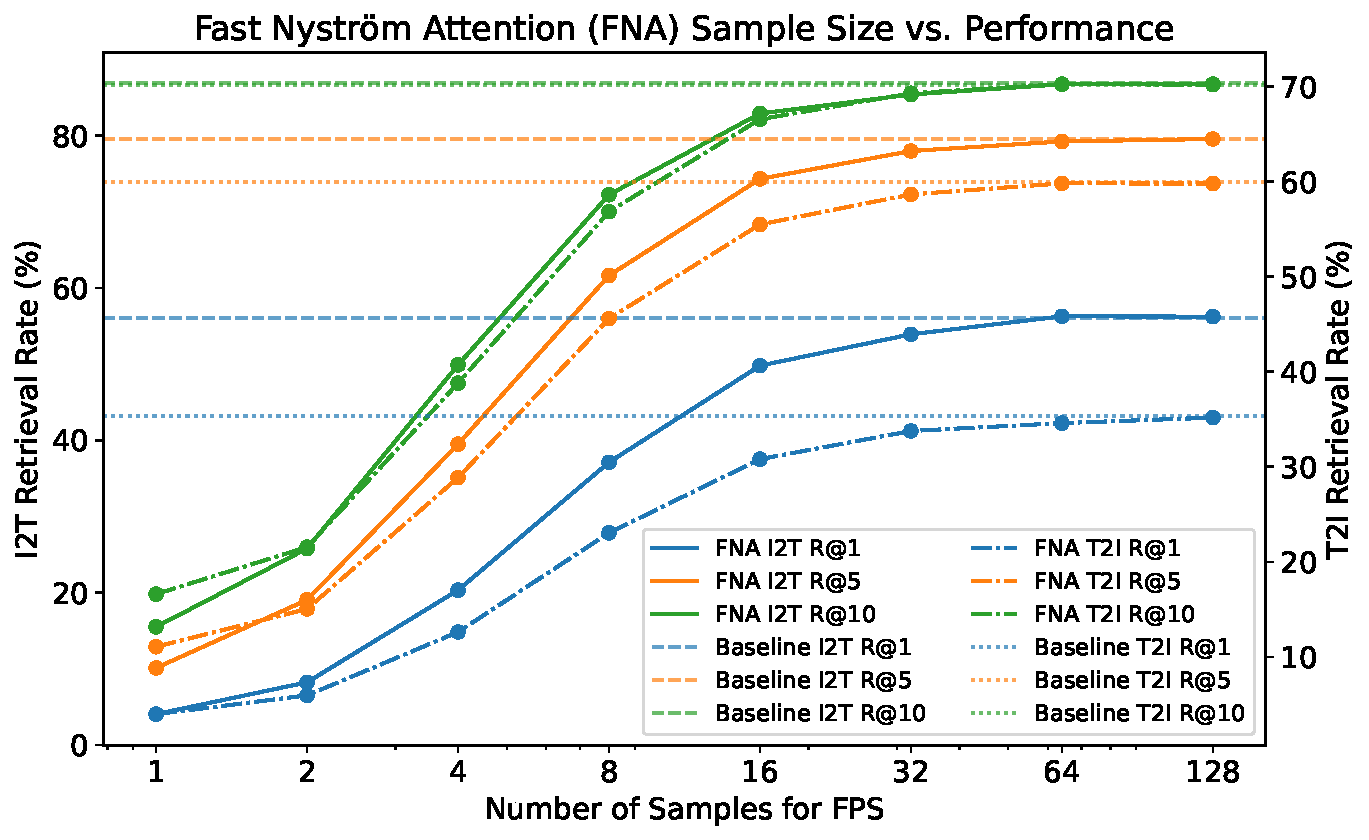
\includegraphics[width=1\linewidth]{figs/fna_sample_size_vs_performance.pdf}
%     \caption{Furthest point sampling (FPS) sample size vs. performance for COCO retrieval with CLIP ViT L-14 at 224x224px input resolution.}
%     \label{fig:fna_sample_size}
% \end{figure}


% \begin{table}[H]
% \centering
% \footnotesize
% \resizebox{\columnwidth}{!}{%
% \begin{tabular}{lcccc}
% \toprule
%  & \multicolumn{2}{c}{Standard Attention} & \multicolumn{2}{c}{Fast Nystro\"m Attention} \\
% Sequence Length & Memory (MB) & Time (ms) & Memory (MB) & Time (ms) \\
% \midrule
% 256 & 133 & 0.8 & 108 & 1.2 \\
% 512 & 257 & 2.1 & 140 & 2.0 \\
% 1,024 & 697 & 5.4 & 204 & 3.4 \\
% 2,048 & 2,376 & 17.5 & 332 & 6.0 \\
% 4,096 & 8,904 & 55.7 & 588 & 11.6 \\
% 8,192 & 34,632 & 201.8 & 1,100 & 22.9 \\
% \bottomrule
% \end{tabular}%
% }
% \caption{Memory consumption and running time results on various sequence lengths. We report the average memory consumption and running time for one input batch (batch size = 8) through a standard self-attention module (from scratch) and our Fast Nystr\"om Attention (sample size = 64). }
% \label{tab:nfa_speed_and_mem}
% \end{table}
% \subsection{Additional Performance Gains}
Vision transformers that incorporate a CLS token often exhibit a subtle separation of information between the CLS and image tokens. To illustrate this, we evaluated a pretrained CLIP ViT L-14 model on ImageNet by fitting a linear probe to different token types at each layer. As shown in Figure \ref{fig:imagenet_lin_probe}, the CLS token initially contains less global semantic information than the average normal tokens as evidenced by lower scores in middle layers; however, it surpasses them in the final layers as it aggregates information for classification. Nevertheless, leftover massive and artifact tokens can interfere with the CLS token’s access to image features, effectively \emph{sinking} attention away. They also introduce noise into the patch representations themselves, degrading performance in both global (\eg, classification, retrieval) and dense tasks (\eg, segmentation).

In practice, we can detect massive and artifact tokens after formation in earlier layers and replace them with nearby normal tokens in the final layers. Applying this masking strategy to CLIP ViT L-14 consistently improves zero-shot retrieval on COCO Captions~\cite{chen2015coco} and Flickr30k~\cite{young2014flickr} (Table~\ref{tab:combined_retrieval}). A similar improvement on image classification and segmentation is shown in Appendix \ref{sec:appendix_results_mask_gains}.



% Interestingly, vision transformers that incorporate a CLS token in their training objectives exhibit a subtle separation of information between the CLS and patch tokens. We evaluated a pretrained CLIP ViT L-14 model on ImageNet by fitting a linear probe to token partitions at each layer. As shown in Figure \ref{fig:imagenet_lin_probe}, in the early and middle layers, the global semantic information needed for classification is consistently lower in the CLS token than the average found in normal or artifact tokens. In the final layers however, the attention from the CLS token to Normal , aggregating global information and surpassing the other token types in accuracy. During this last phase, leftover massive and artifact tokens hinder the flow of information from the patch tokens to the CLS token through both the sinking mechanism and as noise among the patch features. Table \ref{tab:combined_retrieval} summarizes how masking massive and artifact tokens with the nearest Normal token in the last layers of CLIP boost performance in both image and text retrieval on COCO Captions \cite{chen2015coco} and Flickr30k \cite{young2014flickr}. Similarly, this masking strategy increases zero-shot ImageNet accuracy by by a small margin for CLIP (Table \ref{tab:vision_only_results}). 

% For tasks that explicitly rely on patch features—such as semantic segmentation—linear probing of the output features is a common approach. In these scenarios, masking the massive and artifact tokens by replacing them with the nearest normal token effectively cleans the output, removing noise and preserving critical local details. As shown in Figure \ref{fig:dino_clip_artifacts}, this masking strategy enhances the visualization of image features in the final layers of both CLIP and DINOv2 by denoising and boosting contrast between relevant objects. Consequently, these improvements translate into better semantic segmentation performance on VOC2012 \cite{pascal-voc-2012} and ADE20k \cite{zhou2017ade}.







% \begin{figure*}[t]
%     \centering
%     \begin{subfigure}[t]{0.45\linewidth}
%         \centering
%         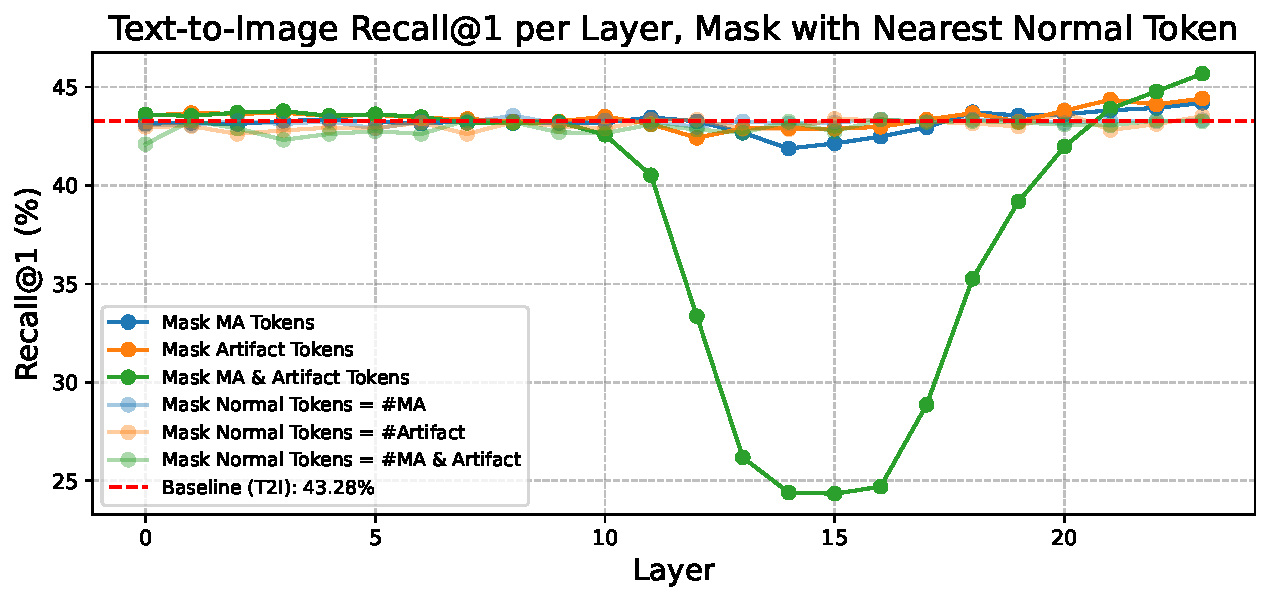
\includegraphics[width=\linewidth]{figs/t2i_replace_with_nearest.pdf}
%         \caption{Add caption for (a)}
%         \label{fig:t2i_replace}
%     \end{subfigure}
%     \hfill
%     \begin{subfigure}[t]{0.45\linewidth}
%         \centering
%         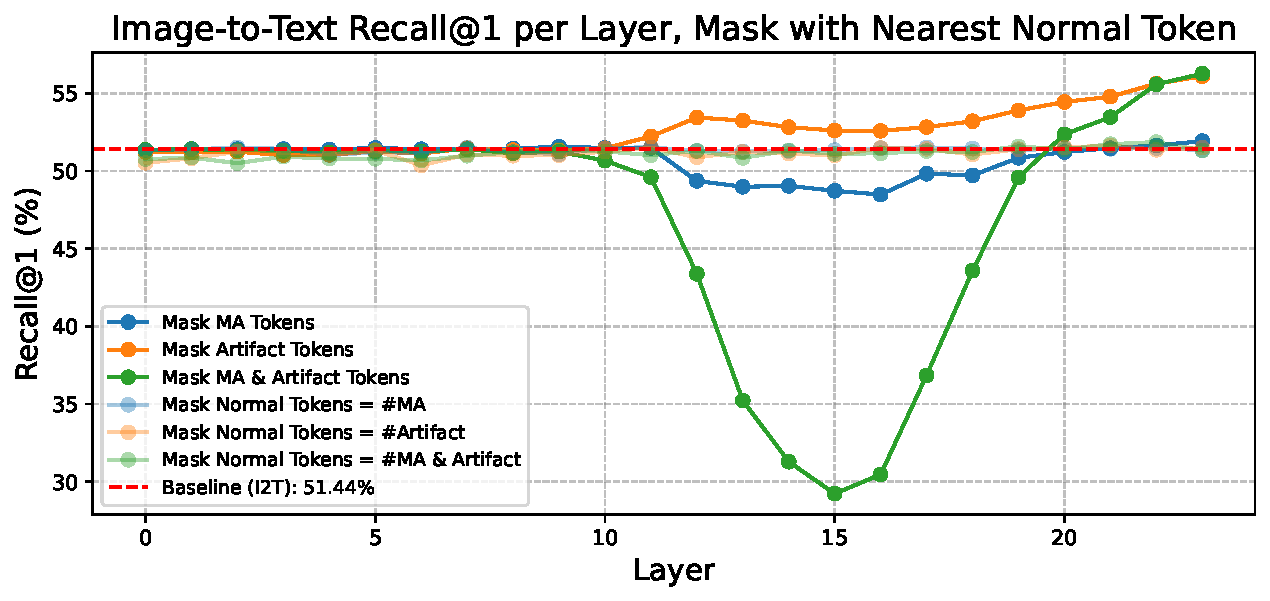
\includegraphics[width=\linewidth]{figs/i2t_replace_with_nearest.pdf}
%         \caption{Add caption for (b)}
%         \label{fig:i2t_replace}
%     \end{subfigure}
    
%     \vspace{1em} % Adjust vertical space between rows if needed
    
%     \begin{subfigure}[t]{0.45\linewidth}
%         \centering
%         \includegraphics[width=\linewidth]{figs/t2i_mask_after_softmax.pdf}
%         \caption{Add caption for (c)}
%         \label{fig:t2i_mask_after}
%     \end{subfigure}
%     \hfill
%     \begin{subfigure}[t]{0.45\linewidth}
%         \centering
%         \includegraphics[width=\linewidth]{figs/i2t_mask_after_softmax.pdf}
%         \caption{Add caption for (d)}
%         \label{fig:i2t_mask_after}
%     \end{subfigure}
%     \caption{Add caption}
%     \label{fig:clip_retrieval_ablation}
% \end{figure*}

% \begin{figure}[ht]
%     \centering
%     \begin{subfigure}[t]{1.0\linewidth}
%         \centering
%         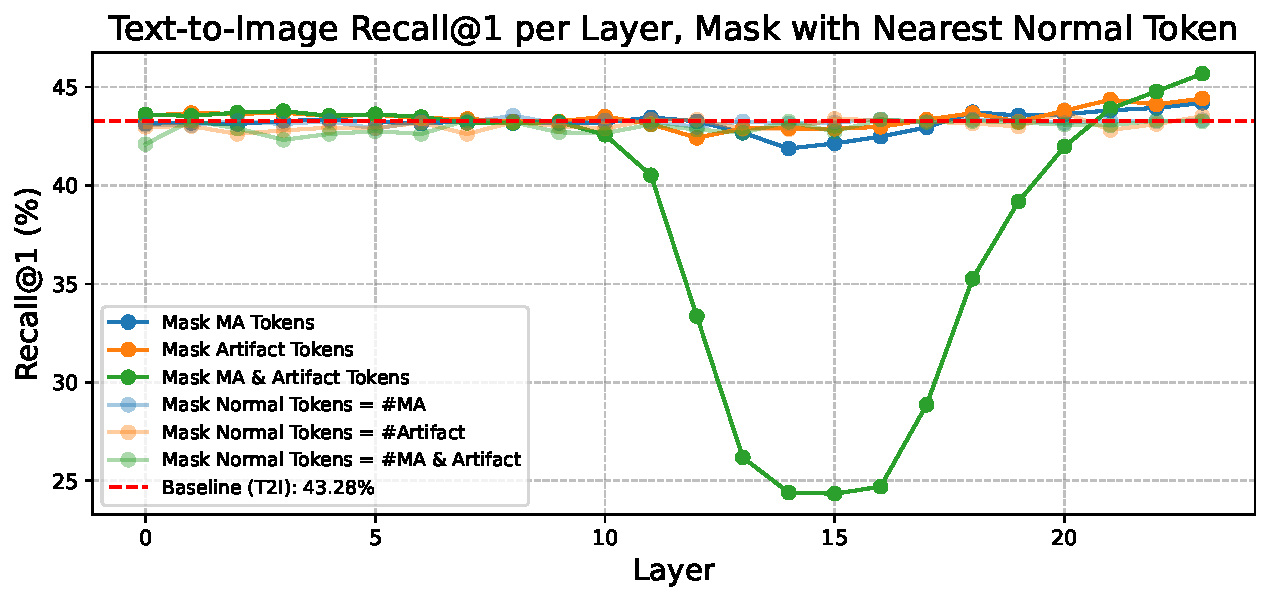
\includegraphics[width=\linewidth]{figs/t2i_replace_with_nearest.pdf}
%         \label{fig:t2i_replace}
%     \end{subfigure}
%     \vspace{0.1cm} % adjust vertical spacing as needed
%     \begin{subfigure}[t]{1.0\linewidth}
%         \centering
%         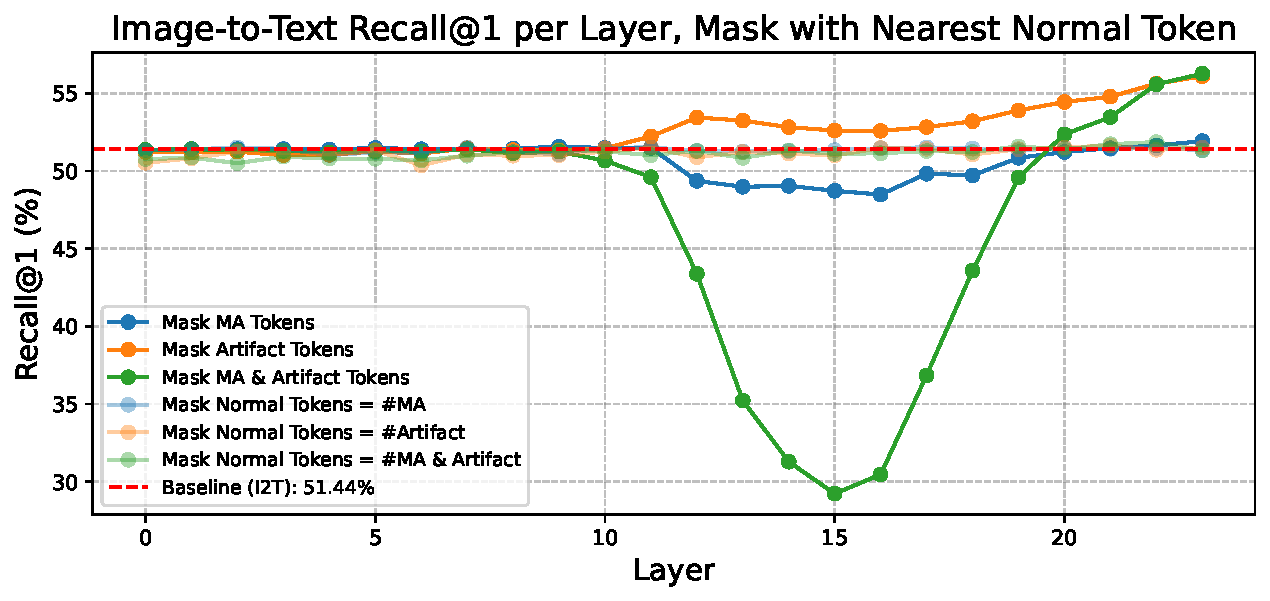
\includegraphics[width=\linewidth]{figs/i2t_replace_with_nearest.pdf}
%         \label{fig:i2t_replace}
%     \end{subfigure}
%     \caption{Zero-shot image and text retrieval ablation performed on COCO with pretrained CLIP ViT L-14 show the effect of masking sink tokens at each layer.}
%     \label{fig:retrieval_ablation}
% \end{figure}


\begin{table}[t]
\centering
\footnotesize
% Subtable (a): Image Retrieval
\begin{subtable}[t]{\columnwidth}
\centering
\resizebox{\columnwidth}{!}{%
\begin{tabular}{lcccccc}
\toprule
 & \multicolumn{3}{c}{COCO} & \multicolumn{3}{c}{Flickr30k} \\
Model & R@1 & R@5 & R@10 & R@1 & R@5 & R@10 \\
\midrule
CLIP & 35.33 & 59.97 & 70.15 & 65.20 & 87.24 & 92.00  \\
CLIP+masking & \textbf{37.47} & \textbf{62.06} & \textbf{72.25} & \textbf{66.96} & \textbf{88.56} & \textbf{93.18} \\
\bottomrule
\end{tabular}%
}
\caption{Image retrieval}
\label{tab:image_retrieval_sub}
\end{subtable}

\vspace{1em}

% Subtable (b): Text Retrieval
\begin{subtable}[t]{\columnwidth}
\centering
\resizebox{\columnwidth}{!}{%
\begin{tabular}{lcccccc}
\toprule
 & \multicolumn{3}{c}{COCO} & \multicolumn{3}{c}{Flickr30k} \\
Model & R@1 & R@5 & R@10 & R@1 & R@5 & R@10 \\
\midrule
CLIP & 56.06 & 79.48 & 86.84 & 85.10 & 97.30 & 99.00 \\
CLIP+masking & \textbf{57.74} & \textbf{79.96} & \textbf{87.40} & \textbf{87.40} & \textbf{97.90} & \textbf{99.10} \\
\bottomrule
\end{tabular}%
}
\caption{Text retrieval}
\label{tab:text_retrieval_sub}
\end{subtable}
\vspace{-1em}
\caption{Zero-shot retrieval results for pretrained CLIP ViT L-14 on COCO \cite{chen2015coco} and Flickr30k \cite{young2014flickr} show performance gains from masking sink tokens at the final layers.}
\label{tab:combined_retrieval}
\end{table}


% \begin{table}[t]
% \centering
% \footnotesize
% \resizebox{\columnwidth}{!}{%
% \begin{tabular}{lcccccc}
% \toprule
%  & \multicolumn{2}{c}{ImageNet} & \multicolumn{2}{c}{VOC2012} & \multicolumn{2}{c}{ADE20k} \\
% Model & Top1 & Top5 & aACC & mIoU & aACC & mIoU \\
% \midrule
% CLIP & 75.96 & 94.82 & 90.33 & 66.60 & 69.55 & 34.84 \\
% CLIP+masking & \textbf{76.26} & \textbf{94.86} & \textbf{90.59} & \textbf{66.96} & \textbf{69.91} & \textbf{35.09} \\
% \midrule
% DINOv2 & \textbf{78.62} & 92.91 & 94.12 & 77.54 & 78.65 & 44.48 \\
% DINOv2+masking & \textbf{78.62} & \textbf{93.06} & \textbf{94.99} & \textbf{79.65} & \textbf{78.76} & \textbf{44.72} \\
% \bottomrule
% \end{tabular}%
% }
% \caption{Vision-only results for pretrained CLIP and DINOv2 ViT L-14. ImageNet \cite{deng2009imagenet} classification evaluation is performed in the zero-shot setting. Segmentation on VOC2012 \cite{pascal-voc-2012} and ADE20k \cite{zhou2017ade} is performed via fitting linear probes to output of the final layers. We show minor but consistent performance gains from masking sink tokens in the final layers. (MOVE TO APPENDIX)}
% \label{tab:vision_only_results}
% \end{table}


